\TUchapter{Results}
\TUsection{Introduction}
The preceding chapters introduced a framework for discrete attack graphs,
a set of enhancements to that framework to improve its modeling capabilities for
discrete systems, and a set of extensions to enable it to model cyber-physical
systems.

This section provides an analysis of the resulting framework (including
a discussion of its performance) and its capabilities (articulating its
contribution to the hybrid systems modeler), as well as a discussion of the
network and system analysis that it enables.
\TUsection{Discrete Capabilities}
Previous chapters articulate the enhancements provided by platform
facts, host processing, and the standard lexicon, which provide conveniences
to the modeler and ease model acquisition from a standard network 
representation. However, further discussion is warranted of the power added
by global exploits and grouping exploits.

In short, globalness applies one exploit to multiple asset 
bindings, whereas grouping applies multiple exploits to the same asset binding.
Consider the goal of modeling a fuzzer or automated attack script that
simultaneously attempts to exploit a variety of common web vulnerabilities on
a form on a web server. A successful buffer overflow may give the attacker
login access to the server; successful cross-site scripting may give the
attacker the ability to spoof messages to users; and a successful SQL injection
attack may give the attacker access to sensitive information. Grouping these
automated attacks together enables the modeler to better capture the behavior
of such a ``script kiddie.''

Consider also the case of executing a denial of service attack on a single
network of arbitrary size by disabling a perimeter device. Such an attack would
be impossible to encode in a single transition without the use of a global
exploit. Such an exploit might appear as in Fig.~\ref{fig:network_dos_global}.

\begin{figure}
\begin{lstlisting}
global exploit kill_router(a, r, h)=
    preconditions:
        platform:r,cpe:/h::VulnerableRouter;
        quality:r,status=up;
        quality:h,status=up;
        topology:a->r,connected_network;
        topology:h->r,connected_local_to_internet;
    postconditions:
        insert quality:r,status=down;
        insert quality:h,status=down;
.
\end{lstlisting}
\caption{Global exploit disabling an entire network}
\label{fig:network_dos_global}
\end{figure}

Additionally, the hybrid extensions also permits the use of
networking concepts such as port number (in which, typically, the use of a
port number 1024 or below requires administrative rights) or latency for the
purposes of modeling certain scenarios on information systems without physical
components.
\TUsection{Hybrid Systems Modeling Capabilities}
The real power of the new extensions show in modeling hybrid systems. For
this discussion it is useful to draw upon the theory of hybrid automata for
hybrid systems. A useful goal is the ability to model any hybrid system
(expressible as a hybrid automaton) in the hybrid attack graph formalism. This
is hindered by two major constraints: the inability to use variables
in the right hand side of precondition and postcondition expressions in
hybrid automata, and the requirement that the time domain be discretized.

\TUsubsection{Classes of hybrid systems modeled by hybrid attack graphs}
\label{sec:hag_ha}
Henzinger and others have articulated a special case of the
hybrid automaton called the linear hybrid automaton~\cite{henzinger1996theory}.
The linear hybrid automaton is a hybrid automaton in which (1) all conditions
in the automaton are boolean combinations of linear inequalities, and (2) all
flow conditions use only free variables from $\dot{X}$. In this case, a linear
inequality is an inequality on linear terms, or linear combinations of
integer constants with real valued variables.

Clearly condition (1) does not hold, because of the lack of variables
on the right hand side of the operators in the attack graph language. However,
the subcase in which the left hand side is the variable in question, and the
right hand side is the constant $k_0$ does.

Condition (2) is more subtle but less restricting. As it permits free
variables only from $\dot{X}$, so long as only one free variable from $\dot{X}$ is
used this is exactly equivalent to the behavior permitted in time evolution
exploit patterns. In the less deterministic (and less common) case in which
multiple free variables from $\dot{X}$ are involved in a flow condition,
the hybrid attack graph language permits an execution that conforms to the
hybrid system specification, but not one that explores all possibilities.
\TUsubsection{Hybrid systems to hybrid attack graph mapping}
The hybrid attack graph permits discrete time
simulation of a small, very well behaved subclass of linear hybrid automata.
Nevertheless, this provides sufficient power to capture a wide variety of
systems. Informally, including a HA in a hybrid attack graph can be 
accomplished using the following general mapping:
\begin{description}
\item[Hybrid automata onto assets] The automaton is represented by an asset.
    Therefore its variables take the form of facts on that asset, its
    conditions take the form of preconditions and postconditions on exploits,
    and events, jumps, and time evolution are done on the exploits.
\item[Control modes onto qualities] The control mode is selected based
    upon a quality on the asset. The mode is implemented by the time
    evolution exploit responsible for that particular asset in that
    particular mode. Control switches are not explicitly encoded but can be
    thought of as part of the exploits that change the asset's mode.
\item[State variables onto qualities] The state variables are encoded
    explicitly as qualities about the asset in the fact base.
\item[Initial conditions onto network model] The initial conditions are
    implemented in the network model initial state.
\item[Jump conditions onto non-time exploits] Jump conditions,
    which select when a mode transition \emph{may} occur, are mapped onto
    the conditions of a non-time exploit, so that they may be fired, but not as
    part of the time stepping.
\item[Invariant conditions onto time exploits] Invariant conditions indicate
    when a mode \emph{must} change in order for the inexorable passage of time
    to proceed. Therefore, these conditions are placed explicitly into time 
    exploits to ensure that they are executed before time may continue to pass.
    Their postconditions include a change of the discrete mode quality.
\item[Flow conditions onto time exploits] Flow conditions, which dictate the
    continuous evolution of the system over time, are implemented as rates of
    change in time exploit postconditions (e.g. \texttt{temp-=5}). Their
    repeated application over discretized time intervals cause the
    simulation of continuous time evolution.
\item[Events onto global groupings] Event labels, which are used to synchronize
    mode transitions between multiple automata, are implemented as global group
    names, which force the globally grouped exploits to fire on the
    synchronized assets simultaneously.
\end{description}

\TUsubsection{Zeno concerns}
Two additional concerns exist, to which brief mention is due: \emph{globally 
zeno} behavior and \emph{isolated zeno} behavior.

Globally zeno behavior occurs in a hybrid attack graph when the
repeated application of non-timed exploits is capable of providing an infinite
transition path in which there are no time 
evolution attacks. That is, a model exhibiting globally zeno behavior not only
generates an infinitely large attack graph, but it also generates one that is
capable of causing the convergence of time, which obviously fails to
capture real world behavior.

Such models are probably (but
not necessarily) ill-formed. Infinitely repeated application of discrete
exploits is a sign of poor modeling decisions: ideally, exploits should not be
applied multiple times to the same assets; if they are (as in the setting of a
mode), they should depend upon either the source mode being different from the
destination mode or else depend upon some other result of time evolution. In the
case of mapping onto hybrid automata, this means that self loops (jumps from a
mode onto itself) need to be addressed with caution.

Isolated zeno behavior, which may also be the sign of an ill-formed model, 
occurs when an otherwise active hybrid asset is not fully covered by the time
exploit group. This may occur legitimately if no continuous evolution is
occuring in the asset's mode, or if (as in the case of the Civic in the
car crash example pictured in Fig.~\ref{fig:fullbunny_two_ag}) the asset is
no longer an active part of the simulation. If this behavior appears, care 
should be given that it is not an oversight on the part of the modeler.
\TUsection{Performance}
Although the purpose of this work is not focused upon the performance of the
generation process, a discussion of the performance of the reference
generator is warranted. This section first
provides an outline of the execution of the generation program, decorated with
the order of magnitude of the asymptotic bound of the execution time at
each step. This is used to provide a bound on the scaling of the generator as
a whole. The next subsection demonstrates the empirical results of a performance
analysis, providing graphical scaling data from code profiling
to confirm the predictions of the outline.

It is worth adding that, although this thesis's reference generator scales 
poorly, a significant amount of the attack graph research community as a whole
focuses specifically upon the performance of their generators. Furthermore, care
has been given that the introduction of continuous values does not alter the
complexity of any step of the generation process. For these reason,
the poor performance of the reference generator is assuaged by the applicability
of the wider attack graph research community's performance results.

Driven by the formal definition of the attack graph domains given in 
Section~\ref{sec:domains} and treating platform facts as just a special case
of qualities, notation will henceforth be as in Table~\ref{table:onotation},
presented in order of appearance in the program outline.

\begin{table}
\centering
\begin{tabular}{r|l}
Domain & Symbol \\ \hline
Facts       & $F = |\mathcal{Q}+\mathcal{T}|$ \\
Fact names  & $f$ \\
Exploits    & $E = |\mathcal{E}|$ \\
Depth       & $d$ \\
Assets      & $A = |\mathcal{A}|$ \\
Qualities   & $Q = |\mathcal{Q}|$ \\
Topologies  & $T = |\mathcal{T}|$ \\
Most preconditions in any exploit & $p$ \\
Most postconditions in any exploit & $P$ \\
Most parameters in any exploit & $a$ \\
Possible asset bindings & $B$ \\
\end{tabular}
\caption{Symbols for the magnitudes of attack graph input domains}
\label{table:onotation}
\end{table}

\TUsubsection{Program Outline and Asymptotic Analysis}
The following outline articulates the order of execution steps in the reference
generator. Each boldface step is decorated with the order of the number of
times that piece of code is executed. Indented steps are substeps, which are
executed on the order of their own decorated order, multiplied by the orders of
each of their parent steps. The outline uses the symbols defined in 
Table~\ref{table:onotation}.

\begin{description}
    \item[Build attack graph] $O(1)$
    \begin{description}
        \item[Load initial state] $O(F)$
        \item[Load exploits] $O(E)$
        \item[Generate attack graph (recursive)] $O(d)$
        \begin{description}
            \item[For each analysis state] $O(states)$
            \begin{description}
                \item[Copy network model] $O(A) + O(F)$
                \item[Get valid attacks] $O(1)$
                \begin{description}
                    \item[For attack in attack bindings] $O(B E)$
                    \begin{description}
                        \item[Validate attack] $O(p)$, which is
                            technically bounded by $O(A^2) \cdot O(F)$
                            but is in practice quite small
                        \item[Process groups and globals] $O(1)$
                    \end{description}
                \end{description}
                \item[For each valid attack] $O(B E)$
                \begin{description}
                    \item[Get successor state] $O(1)$
                    \begin{description}
                        \item[Build network model] $O(A) + O(F)$
                        \item[Add postconditions] $O(P)$, which is
                            technically bounded by $O(A^2 F)$
                            but is in practice quite small.
                    \end{description}
                \end{description}
            \end{description}
        \end{description}
    \end{description}
\end{description}
There are two non-obvious variables included here. One is 
$B$, the possible binding combinations value, which is
actually the result of a permutation operation. This is bounded loosely by
by $O(A!)$ (or $O(A^A)$) and more tightly for a given scenario by 
$O\left(\frac{A!}{(A-a)!}\right)$ (alternatively $O(A^a)$),
where $a$ is the length of the longest parameter list on any exploit pattern.

The other is ``states.'' In this case, it refers to the number of ``analysis states''
in an iteration of the generation function, which is actually defined in terms
of the previous iteration's states. Luckily, we can avoid having to solve for
this quantity by combining the sections ``Generate attack graph (recursive)''
with ``For each analysis state.'' Using the knowledge that the body of that for
loop is reached once and only once for each state generated, the bound for the
number of executions of the combined structure is equivalent to the bound on
the number of states in the attack graph. Because a scenario is not guaranteed
to converge to a closed attack graph, this is necessarily a function of the
maximum depth. Each state may produce up to $B \cdot
E$ new states. This may happen up to $d$ (generation depth) times. Using the
derivation of $B$ from earlier in this section, this means 
that the number of states produced is at worst $(A!E)^{D}$.
More tightly, this is in 
$O\left(\left(\left(\frac{A!}{(A-a)!}\right)E\right)^{d}\right)$.
This controls the scaling behavior of the recursive generator function.

Furthermore, the fact ``count'' should actually be broken up into qualities and
topologies (treating platform facts as special cases of qualities for the
purposes of this analysis), as the possible number of these fact types grow 
with respect to the asset count at different rates. The bound on facts, then,
is actually $O(A \cdot Q + A^2 \cdot T)$.

Refer to Table~\ref{table:onotation}. It
includes $P$ and $p$, which refer to the largest number of pre- and 
post-conditions in any single exploit in the input. These can be bounded (in
practice, very loosely) by $O((AQ + A^2T)(A))$, but this bound is due to the
(never practically implemented for nontrivial $A$) possibility of an exploit
taking every possible asset parameter and operating on every possible quality
and topology for each possible asset combination. Similarly, the number of
parameters in exploit patterns could be bounded loosely by $O(A)$, but this is
not realistic. Therefore, the new $a$, $p$ and $P$ inputs are used instead.
The symbol for the number of fact names, $f$, is used in the next
section to simplify some notation.



The outline
reveals the following bound on the generation process:

$O((EB)^d((A+F) + BEp + BE(A+F+P)))$.

Recall that $B = \frac{A!}{(A-a)!}$, so is in $O(\frac{A!}{(A-a)!})$ 
(more loosely, $O(A^a)$ or $O(A!)$ or
even $O(A^A)$ are also valid), and that $F = AQ + A^2T$ (More loosely, $A^2f$). 
Then the generation process is more precisely in:

$O(((\frac{A!}{(A-a)!}E)^d)((A+AQ + A^2T) + \frac{A!}{(A-a)!}Ep + \frac{A!}{(A-a)!}E(A+AQ + A^2T+P)))$

Switching to the looser bounds of $A$ for $p$ and $P$, $A^A$ for $B$ 
(thereby eliminating $a$), and $A^2f$ for $F$
simplifies the presentation of this expression to a function only of $f$,
$E$, $A$, and $d$. It is already clear that execution time is controlled almost
completely by the growth of $A$ and $d$, but this resultant asymptotic bound for
execution time of the (hybrid) attack graph generation process presents that 
fact quite dramatically:

$O((A^AE)^d((A+A^2f) + A^AEA + A^AE(A+A^2f+A)))$

$= O(fEA^{Ad+A+2})$

$= O(E^{d+1}fA^{A(d+1)+2})$

$\approx O(E^{d+1}fA!^{d})$ (in a mild abuse of notation)

Worst case generation time, then, is expected to grow linearly with fact names, 
polynomially with exploit patterns, exponentially with generation depth (for divergent 
graphs), and factorially with assets. The next sections demonstrate empirically
the effects of generation depth and asset growth on execution time.
\TUsubsection{Execution Time Results}
Two sets of trials serve to demonstrate the scaling behavior of execution time:
on assets, and depth. These were executed using a combination of the 
homogeneous automotive example (in which the only cars are ``Civics'') from
Section~\ref{sec:car} and the RFID example from Section~\ref{sec:rfid}.

\TUsubsubsection{Asset scaling}
The first set of tests, which studies the effect of increasing the number of 
input assets while holding everything else (including depth) constant,
includes both the car and RFID scenarios. Inclusion of additional cars and
tags provides the asset scaling. The RFID scenarios were allowed to continue
until convergence; the car scenarios, which do not converge, were generated
to a depth of 10. Each asset number (from 2 to 6, representing 1 to 5 cars; and
3 to 6, representing 1 to 4 RFID tags) was executed on each scenario 6 times.
The results, showing dramatic exponential behavior, are provided in 
Fig.~\ref{fig:assetperf}. These are graphed on a logarithmic scale with a
reference line of $A^A$ in Fig.~\ref{fig:assetperflog}.

This exponential behavior especially affects hybrid attack graphs with time 
because time group exploits are likely to bind to nearly every permutation of 
asset choices. As an example, observe the large number of permutations of 
bindings of the time group exploits to car assets in 
Fig.~\ref{fig:5car_ag_shallow}.

\begin{figure}
\centering
\includegraphics[width=\textwidth]{perf/asset_time}
\caption{Execution time vs. number of assets}
\label{fig:assetperf}
\end{figure}

\begin{figure}
\centering
\includegraphics[width=\textwidth]{perf/asset_time_log}
\caption{Execution time vs. number of assets (log scale)}
\label{fig:assetperflog}
\end{figure}

\begin{figure}
\centering
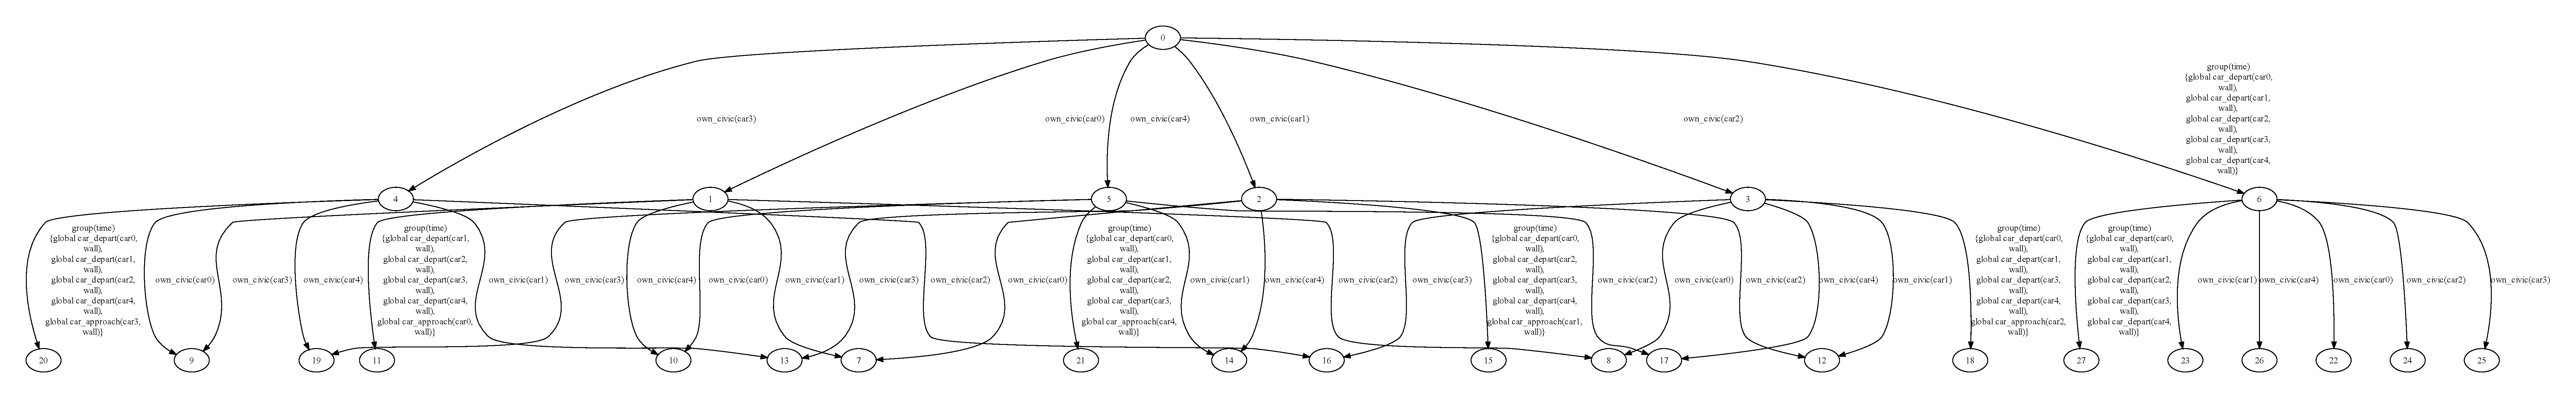
\includegraphics[angle=90,height=0.9\textheight]{fullbunny_s5_d2}
\caption{5-car hybrid attack graph to depth 2}
\label{fig:5car_ag_shallow}
\end{figure}

\TUsubsubsection{Depth scaling}
The second test set, performed by varying the generation depth of the
program, again with 6 trials, serves to illustrate both the exponential growth
of execution time with depth, as well as the difference in the way that depth
affects converging attack graphs (such as the RFID example) and diverging ones
(such as the car example). The graph of this performance is provided in 
Fig.~\ref{fig:depthperf} and on a logarithmic scale in 
Fig.~\ref{fig:depthperflog}.

\begin{figure}
\centering
\includegraphics[width=\textwidth]{perf/depth_time}
\caption{Execution time vs. generation depth}
\label{fig:depthperf}
\end{figure}

\begin{figure}
\centering
\includegraphics[width=\textwidth]{perf/depth_time_log}
\caption{Execution time vs. generation depth (log scale)}
\label{fig:depthperflog}
\end{figure}